
\usetikzlibrary{arrows.meta,calc,patterns,shapes}
\providecommand{\computer}{%
    
\includegraphics[width=1cm]{../common/Noun_project_216.pdf}
}
\providecommand{\switch}{%
    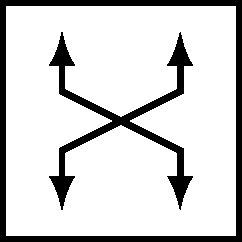
\includegraphics[width=0.9cm]{../common/fig-switch.pdf}
}
\providecommand{\bigswitch}{%
    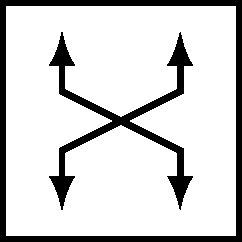
\includegraphics[width=1.4cm]{../common/fig-switch.pdf}
}
\providecommand{\router}{%
    
\includegraphics[width=0.9cm]{../common/fig-router.pdf}
}


\begin{frame}[label=connTwoNet]{connecting two networks}
\begin{tikzpicture}
\tikzset{
    connect/.style={draw,very thick,Latex-Latex},
    computer/.style={inner sep=0mm,outer sep=0mm,execute at begin node={\computer}},
    switch/.style={inner sep=0mm,outer sep=0mm,execute at begin node={\switch}},
    big switch/.style={inner sep=0mm,outer sep=0mm,execute at begin node={\bigswitch}},
    router/.style={inner sep=0mm,outer sep=-2mm,execute at begin node={\router},circle},
    packet/.style={minimum width=.4cm,minimum height=0.2cm,inner sep=0mm,outer sep=0mm,draw},
    packet lg/.style={minimum width=.6cm,minimum height=0.2cm,inner sep=0mm,outer sep=0mm,draw},
    network/.style={draw,cloud,font=\small,aspect=3,inner sep=-.25cm},
    tunnel/.style={dotted,line width=1mm,dotted,blue,Latex-Latex,opacity=0.7},
}
\begin{scope}
    \node[network] (site A) at (0, 0) {company site A};
    \node[network] (site B) at (4, 0) {company site B};
    \node[network,minimum height=1.7cm,minimum width=2.7cm] (internet) at (2, 4)  {
        internet
    };
    \node[router,anchor=south] (A route) at ([yshift=1cm]site A.north) {};
    \node[router,anchor=south] (B route) at ([yshift=1cm]site B.north) {};
    \foreach \x/\y in {site A/A route,site B/B route,A route/internet,B route/internet} {
        \draw[connect] (\x) -- (\y);
    }
    \draw[tunnel]
        (A route.north east) -- ([yshift=-.7cm,xshift=-1cm]internet.center)
            -- ([yshift=-.7cm,xshift=1cm]internet.center) -- (B route.north west);
    \node[draw=red,fill=white,align=center,anchor=north,font=\small,thick] at (2, 5.7) {
        setup tunnel \\
        between disconnected sites
    };
\end{scope}
\node at (2, 6) { actual connections };
\node at (10, 6) { logical connections };
\draw[ultra thick] (6, -1) -- ++ (0, 7);
\begin{scope}[xshift=8cm,name prefix=alt-]
    \node[network] (site A) at (0, 0) {company site A};
    \node[network] (site B) at (4, 0) {company site B};
    \node[network,minimum height=1.7cm,minimum width=2.7cm] (internet) at (2, 4)  {
        internet
    };
    \node[router,anchor=south] (A route) at ([yshift=1cm]site A.north) {};
    \node[router,anchor=south] (B route) at ([yshift=1cm]site B.north) {};
    \foreach \x/\y in {site A/A route,site B/B route,A route/internet,B route/internet} {
        \draw[connect] (\x) -- (\y);
    }
    \node[draw=red,align=center,fill=white,anchor=north,font=\small,thick] at (2, 5.7) {
        as if directly\\
        linked sites
    };
    \draw[connect] (A route) -- (B route);
\end{scope}
\end{tikzpicture}
\end{frame}

